\section{它说了什么？}\label{sec:2}

现在我们来更仔细地考察几何朗兰兹对偶的实际陈述。

\subsection{语言：勇敢新世界的调和分析与泛函分析}\label{sec:2.1}

我们论证过，谱定理关涉一个范畴，即 $\R$ 的酉表示——我们不仅有对象的集合，而且它们还彼此“交谈”。确实，表示论的基本研究对象就是范畴：它们作为群或代数的表示而出现，而目标是以有意义的方式描述它们，正如谱理论用本征空间把带自同态的向量空间搭建起来。

另一方面，\S\ref{sec:1.2} 中谱定理与傅里叶变换之间的类比——其中向量空间扮演数的角色，向量空间族扮演函数或测度的角色——提示我们把范畴本身看作希尔伯特空间的类比物。确实，范畴中的对象有一个“内积”，即它的 Hom 空间。当然，要成为一个希尔伯特空间，远不止一个带内积的集合——我们还有加法与数乘、拓扑与完备性。同样，我们要的不只是一个范畴，而是具有直和之类运算以及某种完备性概念的范畴。在这一类比中，同调代数取代了域 $k$ 上的线性代数：能够施行基本运算的那类性态良好的范畴，我们称之为导出范畴（derived category）（技术性的名称涉及三角 dg 范畴或 $k$-线性稳定 $\infty$-范畴之类的词）。这些基本例子由 $k$-代数的模范畴出发、“对同调代数的运算作完备化”而建成。同伦代数随后为泛函分析中的许多基本构造提供了对应物。

经典调和分析描述函数向量空间在对称群作用下的分解。近几十年来，一种丰富的范畴化调和分析已经浮现：其中函数向量空间被层的导出范畴（即各种取值于向量空间的“函数”）取代。例如，我们把 $z^{s}$ 这样的函数换成它们所满足的微分方程，如 $z\frac{d}{dz}-s$；把梅林变换这样的变换换成范畴上相应的函子。不断壮大的各种层论（又称六函子形式）为形形色色的函数空间提供了对应物。我们把一些松散的类比总结如下：\zhnote{“六函子形式”（six-functor formalism）指一套把层的推前、拉回、张量积、内 Hom、上同调与紧支撑上同调这六个操作公理化、并使之在导出范畴层面相容的形式体系；nLab 词条 \emph{six operations} 列出了这六个操作及其相容关系：\href{https://ncatlab.org/nlab/show/six+operations}{\texttt{https:/\allowbreak{}/\allowbreak{}ncatlab.\allowbreak{}org/\allowbreak{}nlab/\allowbreak{}show/\allowbreak{}six+\allowbreak{}operations}}（最后修订 2026-09-30）。原文所谓“brave new harmonic analysis”正是指：泛函分析里的积分、乘法、函数空间，在层论中分别对应推前／直积分、张量积、层的导出范畴。}

\begin{center}
\renewcommand{\arraystretch}{1.25}
\begin{tabular}{ll}
\toprule
泛函分析 & 范畴化的对应物\\
\midrule
向量空间 & 范畴\\
希尔伯特空间 & 导出范畴\\
算子 & （正合）函子\\
函数 & 层\\
积分 & 推前／直积分\\
乘法 & 张量积\\
函数空间 & 层的导出范畴\\
\bottomrule
\end{tabular}
\end{center}

GLC 的证明要求在一个全新的范畴化背景下，为泛函分析与调和分析的许多经典章节发展出对应物。这解释了本领域论文为何冗长而复杂，但也是这项事业对代数与解析几何、同伦论、数学物理与表示论等更广泛共同体的主要红利之一。由于其技术性，下文将尽量避免这种语言。

\subsection{背景：丛的模空间}\label{sec:2.2}

我们固定一个紧黎曼面（光滑复代数曲线）$C$，以及一个复约化群 $G$——读者不妨就把它取为可逆矩阵群 $\mathrm{GL}_{n}(\C)$，损失不大。我们将聚焦于非分歧的 GLC，即不在 $C$ 上打洞、也不在 $C$ 的点上添加额外数据。这是最基本的情形，也是已经被证明的情形，尽管大部分一般想法都有分歧版本。

主要研究对象是 $\Bun_{G}(C)$，即 $C$ 上代数（或全纯）$G$-丛的模空间（当 $C$ 不言自明时记作 $\Bun_{G}$）。这是代数几何中参数化 $C$ 上主 $G$-丛（即当 $G=\mathrm{GL}_{n}$ 时的秩 $n$ 向量丛）的对象。这意味着它不仅由点、而且由所有映入它的映射来定义——给出从簇 $S$ 到 $\Bun_{G}(C)$ 的映射，等同于给出 $S\times C$ 上的一个 $G$-丛。换言之，它是拓扑中分类空间在代数几何中的版本——具体说，它是从 $C$ 到 $G$ 的分类空间的代数映射空间。

这里先剧透一下结局：从几何（即点或经典力学）的角度看，空间 $\Bun_{G}$ 显得有些繁复巴洛克；但从它的线性化（即调和分析或量子力学）的角度看，它会显得漂亮得多。

\subsubsection{阿贝尔情形：雅可比簇}\label{sec:2.2.1}

要理解 $\Bun_{G}$，先考虑 $G=\mathrm{GL}_{1}$ 的情形，其研究可追溯到 Abel、Jacobi 与 Riemann。此时 $G$-丛与 $C$ 上的全纯线丛是同一份数据。经典地，线丛（或更确切地说，其全纯截面）由 $C$ 上的除子——$C$ 的点的整系数线性组合——给出，它确定一个在指定点至多取指定阶极点、至少取指定阶零点的亚纯函数空间。两个除子描述同一个线丛，当且仅当它们相差 $C$ 上某个实际有理函数给出的除子。

线丛的模空间 $\Bun_{\mathrm{GL}_{1}}(C)=\mathrm{Pic}(C)$ 就是 $C$ 的 Picard 群。关键事实已经出现：Picard 群在\emph{线丛张量积}这一运算下是一个阿贝尔群。更具体地，群结构由除子相加给出：$\mathrm{Pic}(C)$ 是除子群（以 $C$ 的点为基的自由阿贝尔群）对“整体”关系（来自亚纯函数的除子）的商。此外这个群有非常简单的描述：它是整数（给出除子的次数）与 $C$ 的雅可比簇的乘积
\[
\mathrm{Pic}(C)\;\cong\;\Z\times \mathrm{Jac}(C),
\]
而 $\mathrm{Jac}(C)$ 作为拓扑群是维数等于 $C$ 的亏格 $g$ 的环面，$\mathrm{Jac}(C)\cong(S^{1})^{2g}$。

\subsubsection{$\Bun_{G}$ 长什么样？}\label{sec:2.2.2}

现在来考虑 $G$-丛模空间的几何；对 $G=\mathrm{GL}_{n}$，它就是参数化 $C$ 上所有秩 $n$ 全纯向量丛的空间。图~\ref{fig:2} 给出了 $\Bun_{G}$ 的一幅图景。

\begin{figure}[tbp]
\centering
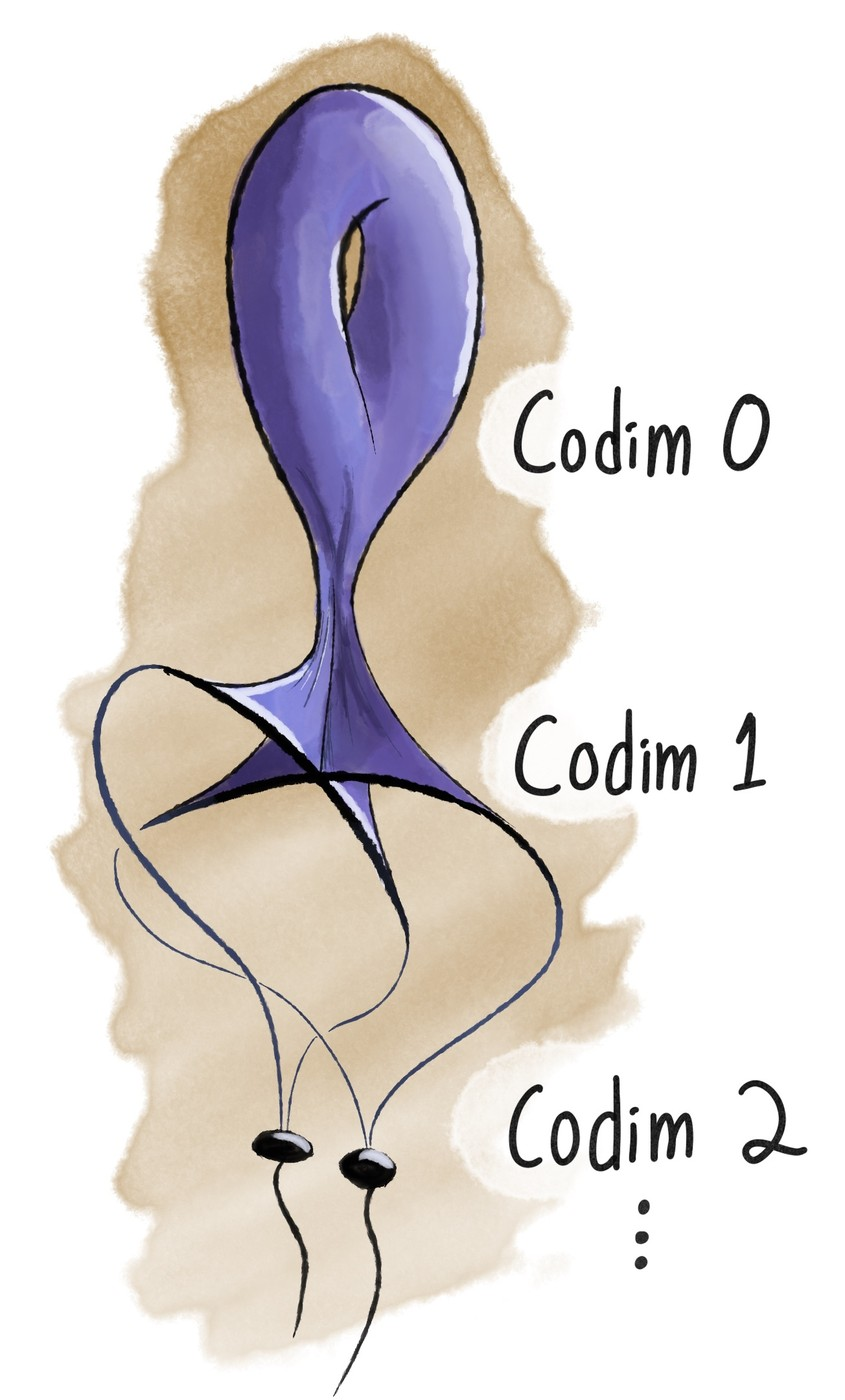
\includegraphics[width=0.34\linewidth]{figures/fig2.jpg}
\caption{$G$-丛模栈 $\Bun_{G}$ 的一幅图景：无限的“尾巴”由自同构越来越多的丛组成，核心则是半稳定丛。（插图：Elliot Kienzle）}\label{fig:2}
\end{figure}

这个空间比雅可比簇难对付得多：

\begin{itemize}
\item 第一，秩 $n$ 丛的集合上没有自然的乘法（对其他 $G$ 也没有），所以 $\Bun_{G}$ 不是群，更不是阿贝尔群。
\item 第二，$\Bun_{G}$ 不是簇，而是模栈（stack）——经典簇与分类空间的混合体。诗意地说，它是一个“点带有自同构群”的簇，因为丛可能有值得注意的自同构群。对雅可比簇而言，忽略这些自同构无伤大雅：所有线丛的自同构群都是同一个 $\C^{\times}$（于是只不过在 $\mathrm{Pic}(C)$ 连通分支的 $\Z$ 之外多一个同等的因子）。
\item 第三，与雅可比簇不同，$\Bun_{G}$ 的连通分支不是（拟）紧的。它包含一条无限的“尾巴”，由自同构越来越多的丛组成，这些丛通过在越来越大的次数范围内逐次扩张线丛而得到。这与模曲线（如椭圆曲线的模空间 $\mathbb{H}/\mathrm{PSL}_{2}\Z$）的尖点（以及由此产生的非紧性）密切类比。
\end{itemize}

在代数几何中，通常的做法是砍掉不稳定丛的尾巴，然后把半稳定丛的开核心坍缩到射影簇上——即几何不变量理论给出的半稳定 $G$-丛模概形。然而对 GLC 而言，保留带着全部“瑕疵”的完整 $\Bun_{G}$ 至关重要。第一，我们做的是表示论，丢弃内部对称群违背这门学科的全部精神；第二，半稳定丛构成的簇本身可能奇异（$\Bun_{G}$ 则不然），更关键的是，它的对称性更少：它不被 Hecke 对应（\S\ref{sec:3.1}）保持，而后者正是 Langlands 纲领最本质的特征。所幸尾巴具有良好的归纳结构，与核心的不可约本性形成对照：最“不紧”的部分纤维化到 $G$ 的极大环面的丛空间 $\Bun_{T}$ 上，而后者是若干 Picard 群的乘积。换言之，在尾巴的远端，丛由线丛的逐次扩张给出。一般地，尾巴类似地与其他 Levi 子群的丛相联系（在 $\mathrm{GL}_{n}$ 情形即分块对角矩阵——也就是低秩向量丛的逐次扩张）。

\subsubsection{除子？}\label{sec:2.2.3}

模空间 $\Bun_{G}$ 享有一个重要而微妙的对应物，可与用除子具体描述 $\mathrm{Pic}(C)$、用取指定零点与极点的函数描述线丛截面相类比。这就是：任何丛都可以在有限多个点之外被平凡化。于是，丛可以由“这种平凡化在每个这样的点附近如何失效”来描述。刻画这种失效的不再是一个整数，而是环路群
\[
\LG=\mathrm{Map}(D^{\times},G)
\]
（从去心圆盘映入 $G$ 的映射构成的环路群）对子群 $\LGp=\mathrm{Map}(D,G)$（能延拓到圆盘上的映射）的一个陪集。这个陪集空间 $\Gr=\LG/\LGp$ 就是仿射 Grassmannian（affine Grassmannian），即通常 Grassmannian 在环路群这一无穷维背景下的对应物。于是，我们可以这样指定一个丛：在曲线上指定有限多个点、并在每点标以仿射 Grassmannian 中的一个点（这是除子的类比），再对 $C$ 到 $G$ 的有理映射的作用取商（这是 $C$ 上有理函数的除子的类比）。因此 $\Bun_{G}$（像更熟悉的模曲线一样）有一个数论学家才熟悉的“阿代尔”描述，即双陪集空间
\[
\Bun_{G}=G(F)\backslash G(\mathbb{A}_{C})/G(\mathcal{O}_{\mathbb{A}_{C}})
\]
（这里 $F$ 是 $C$ 上的有理函数域）。这看起来笨重，却让人更深入地理解 $\Bun_{G}$ 的对称性。\zhnote{阿代尔描述与 Weil 单值化定理是同一个陈述：把 $G$-丛在有限多个点外平凡化，用 $G(F)$ 的作用把这些平凡化粘起来，剩下的自由度正是 $\prod'_{x}G(\C((z_{x})))$ 模 $\prod_x G(\C[[z_x]])$。nLab 词条 \emph{Weil uniformization theorem} 给出该双陪集分解的精确定义与它在几何类域论中的用法：\href{https://ncatlab.org/nlab/show/Weil+uniformization+theorem}{\texttt{https:/\allowbreak{}/\allowbreak{}ncatlab.\allowbreak{}org/\allowbreak{}nlab/\allowbreak{}show/\allowbreak{}Weil+\allowbreak{}uniformization+\allowbreak{}theorem}}（最后修订 2023-04-04）。}

对半单群 $G$（例如 $\mathrm{SL}_{n}$，即考虑行列式平凡的向量丛），这一描述有一个不那么“民主”却高效得多的变体。固定一点 $x\in C$，则 $\Bun_{G}$ 可以写成类似局部对称空间、类比于模曲线 $\Gamma\backslash\mathbb{H}=\Gamma\backslash \mathrm{SL}_{2}\R/\mathrm{SO}(2)$ 的形式：
\[
\Bun_{G}(C)=G(C\setminus x)\backslash \LG/\LGp,
\]
即单个仿射 Grassmannian 对从去心曲线映入 $G$ 的映射群取商。

\subsubsection{物理视角}\label{sec:2.2.4}

稍稍绕个弯：我要提一句，$\Bun_{G}$ 与黎曼面上 Yang–Mills 泛函的研究密切相关~[AB83]。最著名的结果是：半稳定 $G$-丛的模空间（由 Narasimhan–Seshadri 定理）作为 $C$ 上所有 $G$-规范场（联络）空间中 Yang–Mills 泛函的极小值空间出现。然而 Yang–Mills 泛函的临界点也包含不稳定丛，而该泛函的 Morse 理论控制着整个空间 $\Bun_{G}$ 的拓扑。于是 $\Bun_{G}$ 自然地出现在 $C$ 上量子 Yang–Mills 理论的研究中。这一关系正是 Langlands 纲领与规范理论之间联系的核心。

\subsection{谱侧}\label{sec:2.3}

GLC 的另一侧是 Langlands 参数空间，即 $C$ 上 $\Gd$-局部系统的空间 $\Loc_{\Gd}(C)$。这些空间扮演谱定理中频率或颜色空间 $\R_{t}$ 的角色，其点标记所有可能的“颜色”（本征值）。我们将在 \S\ref{sec:3.5} 中看到 Langlands 参数如何从 $\Bun_{G}$ 上调和分析的研究中作为“答案”有机地出现。

局部系统主要有两种风味，对应于傅里叶理论中对平移与微分的侧重：

\begin{itemize}
\item \textbf{Betti（群）版本}：$\Loc^{\Betti}_{\Gd}$ 本质上就是熟悉的特征簇（character variety），参数化 $C$ 的基本群映入 $\Gd$ 的表示（即当 $G=\Gd=\mathrm{GL}_{n}$ 时的 $n$ 维表示）。它是所有同态 $\pi_{1}(C)\to\Gd$ 构成的（轻度奇异的）仿射簇对 $\Gd$ 的（栈意义上的）商。具体地，对亏格 $g$ 的 $C$，可写
\[
\Loc^{\Betti}_{\Gd}(C)=\Bigl\{A_{1},B_{1},\dots,A_{g},B_{g}\in\Gd:\ \prod_{i=1}^{g}[A_{i},B_{i}]=1\Bigr\}\big/\Gd.
\]
于是对 $G=\Gd=\mathrm{GL}_{1}$ 这不过是 $(\C^{\times})^{2g}$\anote{更确切地说，还要模去自同构的栈性 $\C^{\times}$，并作某种“导出修正”以计入其定义方程的非横截性。}；而对亏格 $1$、$G=\Gd=\mathrm{GL}_{n}$，这是交换矩阵的共轭类空间。与标准特征簇概念的区别在于：正如 $\Bun_{G}$ 的情形，我们不仅记录点，还记录自同构——即考虑局部系统的栈，而不把它坍缩为底层的簇。
\item \textbf{de Rham（李代数）版本}：$\Loc^{\dR}_{\Gd}$ 参数化带平坦联络（flat connection）的 $\Gd$-丛，即向量场的李代数（而非基本群）的作用。于是对 $G=\Gd=\mathrm{GL}_{n}$，这是秩 $n$ 平坦向量丛的模空间。它（忘掉联络后）构成 $\Bun_{\Gd}$ 的某个拟紧开子集上的仿射丛（事实上它构成 $\Bun_{\Gd}$ 的余切丛的一个扭曲版本）。
\end{itemize}

平坦联络定义了平行移动的概念，即其单值性，从而定义了 $\pi_{1}$ 的一个表示。因此 $\Loc_{\Gd}$ 的 Betti 与 de Rham 两个版本在解析意义下相同，在代数意义下却不同——过渡到平行移动（解微分方程）是某种指数映射。例如对亏格 $1$ 的 $\mathrm{GL}_{1}$，前者是 $(\C^{\times})^{2}$，后者是椭圆曲线上的一个 $\C$-丛（一个著名的非仿射曲面，Serre 曾讨论过）。换言之，就点（或无穷小形变）而言两者无法区分，但在考虑局部系统的族时就必须小心。

下文将默认使用中性的记号 $\Loc_{\Gd}$ 表示两种风味的特征簇，凡可能时就隐去区别。

\subsection{几何类域论，或 $\mathrm{GL}_{1}$ 的 GLC}\label{sec:2.4}

让我们（重新）考虑雅可比簇 $\mathrm{Jac}(C)$，即 Picard 群 $\mathrm{Pic}(C)=\Bun_{\mathrm{GL}_{1}}(C)$ 的连通分支。它是阿贝尔群，因此可以在其上做傅里叶理论。具体说，我们可以把 \S\ref{sec:1.3} 的梅林变换描述本质上重复 $2g$ 次。代替可逆算子（即 $\Z$ 的表示）的谱定理，我们考虑 $2g$ 个彼此交换的可逆算子，即 $\Z^{2g}\cong\pi_{1}(\mathrm{Jac}(C))$ 的表示。可以把这些算子重新解释为雅可比环面 $\mathrm{Jac}(C)\cong(S^{1})^{2g}$ 上某个局部系统的单值性——即向量值函数沿 $2g$ 个方向可能的多值性。从谱的角度看，这 $2g$ 个交换算子描述 $2g$ 元洛朗多项式环 $\C[z_{1}^{\pm1},\dots,z_{2g}^{\pm1}]$ 上的一个模，或者更具启发性地，描述一族联合本征空间的代数族，即 $(\C^{\times})^{2g}$ 上的一个拟凝聚层。

另一方面，$(\C^{\times})^{2g}\cong\Loc_{\mathrm{GL}_{1}}(C)$\anote{同样忽略自同构的 $\C^{\times}$。} 是 $C$ 的秩一特征簇——即对 $C$ 中每个环路给一个纯量扭曲的数据。结果是一个等价，即 $\mathrm{GL}_{1}$ 的 Betti GLC：
\[
\Loc(\mathrm{Jac}(C))=\Rep(\Z^{2g})\;\overset{L}{\longleftrightarrow}\;\QCoh\bigl((\C^{\times})^{2g}=\Loc_{\mathrm{GL}_{1}}(C)\bigr).
\]
这个等价具有“傅里叶”性质：用雅可比簇的群结构作平移，被送到乘法（模的张量积）。虽然我们对等价的描述没有用到曲线的任何几何，$L$ 却满足一个自然的几何相容性。由 Abel–Jacobi 映射（即把点看作除子\anote{这个嵌入自然地落在次数为 $1$ 的分支 $\mathrm{Pic}^{1}(C)$ 中，但我们可以减去 $C$ 中一个选定的参考点，把它下移到 $\mathrm{Jac}(C)=\mathrm{Pic}^{0}(C)$，从而得到经典的 Abel–Jacobi 映射。}）给出的包含 $C\hookrightarrow \mathrm{Jac}(C)$ 在阿贝尔化意义下等同了基本群
\[
\pi_{1}(C)^{\mathrm{ab}}\cong\pi_{1}(\mathrm{Jac}(C)),
\]
而 $L$ 把 $\mathrm{Jac}(C)$ 上的秩一局部系统 $E$ 送到 $C$ 上相应的秩一局部系统处的摩天楼 $\OO_{AJ^{-1}(E)}$。这个性质正是（非分歧）几何类域论的特征性质：$L$ 让我们把 $\mathrm{Jac}(C)$ 的覆盖空间与 $C$ 的阿贝尔覆盖空间等同起来，并与 Abel–Jacobi 映射相容。\zhnote{几何类域论是 GLC 在 $G=\mathrm{GL}_{1}$ 时的情形，其经典形式即 Abel–Jacobi 映射给出的 $\mathrm{Pic}^{0}(C)\cong \Loc_{\mathrm{GL}_{1}}(C)$；nLab 词条 \emph{geometric class field theory} 把它表述为“曲线的基本群（阿贝尔化）与其 Picard 簇的基本群之等同”，并指出这正是高维几何 Langlands 的出发点：\href{https://ncatlab.org/nlab/show/geometric+class+field+theory}{\texttt{https:/\allowbreak{}/\allowbreak{}ncatlab.\allowbreak{}org/\allowbreak{}nlab/\allowbreak{}show/\allowbreak{}geometric+\allowbreak{}class+\allowbreak{}field+\allowbreak{}theory}}（最后修订 2025-05-11）。}

\subsubsection{D-模与 de Rham 共形场论}\label{sec:2.4.1}

与梅林变换一样，几何类域论也有 de Rham 版本。这里我们研究的不是局部系统，而是雅可比簇上的 D-模（D-module）。先提三种看待簇 $X$ 上 D-模 $\Dmod(X)$ 的方式：

\begin{itemize}
\item 在仿射簇 $X$ 上，D-模就是 $D(X)$——系数为多项式的微分算子环——上的模。当 $X$ 非仿射时（如我们关心的 $\mathrm{Jac}(X)$），多项式函数不够多，于是使用层论语言：D-模是对 $X$ 的开子集指派这样的模、并在重叠处给出等同的汇集。
\item 通过把 D-模用生成元与关系表示，可以重新解释为系数为多项式的线性偏微分方程组；同样，我们考虑开片上的这样的方程组，并在重叠处作等同。
\item D-模带有（多项式函数层）$\OO_{X}$ 的作用，也带有向量场李代数的作用，二者通过 Leibniz 法则相容。换言之，它是一个带有微分概念（即平坦联络）的拟凝聚层（向量空间的代数族）。
\end{itemize}

把 D-模看作以其解出现的广义函数的范畴化身是有益的，正如我们把 $\C^{\times}$ 上的方程 $z\frac{d}{dz}-s$ 看作其解 $z^{s}$ 的化身。我们将要寻找的单色 D-模（特征层或本征层）正是特殊函数的化身，并分享后者的许多丰富性质。

在雅可比簇上的所有 D-模中，有一类特殊的：带平坦联络的线丛。它们与 $\mathrm{Jac}$ 上的秩一局部系统一一对应，从而（由 Betti 等价）与 $C$ 上的秩一局部系统一一对应，最终与 $C$ 上带平坦联络的线丛一一对应。具体地，这个双射由在 Abel–Jacobi 映射下限制到曲线上给出。我们可以把这个双射解释为：把 $\mathrm{Jac}$ 上的一个 D-模对应到 de Rham 特征簇 $\Loc^{\dR}_{\mathrm{GL}_{1}}(C)$ 上相应点处的摩天楼。Laumon 与 Rothstein~[Lau96, Rot96] 证明了这一对应可以延拓为等价，即 $\mathrm{GL}_{1}$ 的 de Rham GLC：
\[
\Dmod(\mathrm{Jac}(C))\;\overset{L}{\longleftrightarrow}\;\QCoh\bigl(\Loc^{\dR}_{\mathrm{GL}_{1}}(C)\bigr),
\]
并满足与 Betti 版 $L$ 平行的类傅里叶性质。这个等价不如其 Betti 版本初等，部分原因是情形不那么仿射——两侧都不能简单地由单个环上的模给出。确实，该等价只在导出范畴层面成立：它是代数几何中典型的导出等价——Mukai 关于对偶阿贝尔簇上拟凝聚层导出范畴的著名傅里叶变换——的加强版本。尽管如此，对“一半”参数它可以变得非常具体而初等，这些参数平行于梅林变换情形中的基本微分方程 $z\frac{d}{dz}-s$。也就是说，我们可以（不用任何层论）通过指定所有全纯向量场的作用，在 $\mathrm{Jac}$ 上写出显式的一阶微分方程：
\[
t_{\xi_{i}}f=\mu_{i}f,\qquad i=1,\dots,g.
\]
它们对应于平凡线丛上所有平坦联络构成的 $g$ 维族 $d-\omega$，其中 $\omega$ 是 $C$ 上的全纯微分形式。

\subsection{终于，GLC}\label{sec:2.5}

现在我们可以描述 GLC 了——它是上一节几何类域论的非阿贝尔推广。GLC 通过线性化、即建立谱分解问题来研究模空间 $\Bun_{G}$。我们要作谱分解的对象——我们的“范畴化函数空间”——将是 $\Bun_{G}$ 上特定类型的向量空间层。$\Bun_{G}(C)$ 上的层可以看作 $G$ 的表示的 $\C$-类比：确实，如果把 $C$ 换成一个点，$G$-丛的栈就变成带 $G$-对称性的单点，其上的向量空间层正是 $G$ 的线性表示。

那么我们要考虑的是哪一类表示论，即自守层？主要有两种风味，de Rham 与 Betti，分别平行于谱定理用自伴算子（微分）与酉表示（平移）所作的表述：

\begin{itemize}
\item \textbf{de Rham（李代数）版本}：考虑 $\Bun_{G}$ 上的 D-模 $\Dmod(\Bun_{G})$。与任意簇上的 $\Dmod(X)$ 一样，它们定义为坐标片（即参数化 $C$ 上 $G$-丛族的仿射簇）上环 $D$ 的模（或线性偏微分方程组）的相容汇集。
\item \textbf{Betti（群）版本}：这里改而研究可构造层（constructible sheaf），即带沿道路平行移动数据的向量空间族。最基本的例子是局部系统，即 $\pi_{1}$ 的表示，它们来自求解平坦联络的平行移动问题（即描述单值性）。但在 $\Bun_{G}$ 的情形（不同于我们研究梅林变换或雅可比簇时），还需要允许更奇异的对象：只要求平行移动在“多数”方向上可逆。这样的对象出现在求解带特征方向的偏微分方程时，这些特征方向阻碍 Cauchy 问题的局部可解性。究竟允许哪些奇异性（沿幂零方向），其精确选择由表示论中的经验所指引，可追溯到 Harish-Chandra 与 Lusztig 分别关于李群表示与有限群表示之特征的工作，我们将在 \S\ref{sec:4.2} 中讨论。所得的范畴记作 $\Shv_{\Nilp}(\Bun_{G})$。
\end{itemize}

为避免记号累赘，除需要更明确交代背景之处，我们将把两个范畴都简记为 $\Shv(\Bun_{G})$。

主角既已登场，现在可以陈述 GLC 了：

\begin{theorem*}[GLC，[GR24a, ABC+24b, CCF+24, ABC+24a, GR24b]]\label{thm:glc}
存在范畴等价
\[
\Shv(\Bun_{G})\;\simeq\;\QCoh(\Loc_{\Gd}),
\]
de Rham 与 Betti 两种背景均成立，分别是~[BD, AG15] 与~[BZN18] 中的猜想。
\end{theorem*}

换言之，$\Bun_{G}$ 上的自守层——微分方程系统或其拓扑单值性数据——具有谱分解，可分解为 $C$ 的相应形式 $\Gd$-特征簇上的向量空间代数族。等价地，$\Bun_{G}$ 上有一族特殊的层，即单色对象或本征层，由 $\Loc_{\Gd}$ 的点参数化；而所有层都可以唯一地写成诸本征层的叠加。

几点简注：第一，如上陈述的定理并不完全正确——由于空间 $\Loc_{\Gd}$ 的奇异性，我们需要修改“代数族”的概念，把 $\QCoh$ 扩大为更奇异的变体 $\IndCoh_{\Nilp}$，见 \S\ref{sec:5.1}。\zhnote{$\IndCoh$（归纳凝聚层）与 $\QCoh$ 的差别在于：$\QCoh$ 只记录“函子性”中的拉回，而 $\IndCoh$ 同时记录推前与反常推前，因而能容纳奇异簇上的“错维”层。nLab 词条 \emph{ind-coherent sheaves} 给出其定义（$\IndCoh(X)$ 由有界凝聚层的归纳极限、再对拟凝聚层作某种完备化得到）以及与 $\QCoh$ 的比较：\href{https://ncatlab.org/nlab/show/ind-coherent+sheaves}{\texttt{https:/\allowbreak{}/\allowbreak{}ncatlab.\allowbreak{}org/\allowbreak{}nlab/\allowbreak{}show/\allowbreak{}ind-coherent+\allowbreak{}sheaves}}（最后修订 2015-10-05）。原文下标 $\Nilp$ 指“幂零奇异支撑”，见 \S\ref{sec:4.2}。}

第二，出于“泛函分析”的目的，我们处处都必须在导出范畴中工作——尽管这个等价惊人地接近于保持更熟悉的阿贝尔层范畴（特别是，本征层本身确实是层，而非层的复形~[FrR25]）。

第三，如上陈述的定理类似于把谱定理表述为两侧之间的抽象匹配，却完全没有刻画它（不像我们在阿贝尔情形中借助 Abel–Jacobi 相容性所作的那样），也没有指明它与实际本征值的联系——换言之，我们仍然遗漏了整个事业的要旨：这个等价必须对角化某个东西。这是我们下一个话题。
